\documentclass[11pt,aspectratio=169]{beamer}

\usepackage{booktabs}
\usepackage{hyperref}
\usepackage{multirow}
\usepackage{xcolor}

\usetheme[titleformat=smallcaps,progressbar=frametitle]{metropolis}
\definecolor{UTburnt}{HTML}{BF5700}
\definecolor{LBJnavy}{HTML}{172A46}
\setbeamercolor{alerted text}{fg=UTburnt}
\setbeamercolor{frametitle}{bg=LBJnavy,fg=white}
\setbeamercolor{progress bar}{fg=UTburnt,bg=gray!25}

\graphicspath{{assets/}}
\author{Sergio I. Garc\'ia-R\'ios}
\title{Introduction to the Course}
\subtitle{Data Analysis for Public Policy}
\institute{PA 311N: Undergraduate Quantitative Methods\\LBJ School of Public Affairs}
\date{Fall 2026}

\begin{document}
\maketitle

\section{General information}

\begin{frame}{Teaching team and weekly rhythm}
\begin{itemize}
  \item Professor: Sergio I. Garc\'ia-R\'ios
  \item Teaching assistant: Sarah Traore
  \item Monday: lecture and statistical reasoning
  \item Wednesday: guided lab in R
  \item Friday: review, troubleshooting, and \textbf{On Your Own} support
\end{itemize}
\vspace{0.4em}
\alert{Office hours:} Sergio by appointment; Sarah Wednesday 12:30--2:00 and Friday 11:00--12:30.
\end{frame}

\begin{frame}{Required materials}
\begin{itemize}
  \item \textit{OpenIntro Statistics}, 4th edition: \url{https://www.openintro.org/book/os/}
  \begin{itemize}
    \item Freely available online; an inexpensive print edition is optional.
  \end{itemize}
  \item R, RStudio Desktop, and Quarto
  \item A laptop for guided labs
  \item Optional calculator
\end{itemize}
\end{frame}

\begin{frame}{Course website}
\centering
{\Large Undergraduate Quantitative Methods}\par
\vspace{0.4em}
{\large Data Analysis for Public Policy}\par
\vspace{0.8em}
\url{https://garciarios.github.io/lbj_ug_quant/}
\end{frame}

\section{Course structure}

\begin{frame}{Learning sequence}
\begin{enumerate}
  \item Data, measurement, and exploratory analysis
  \item Probability and distributions
  \item Sampling, uncertainty, and foundations for inference
  \item Hypothesis testing and comparisons
  \item Correlation and regression
  \item Communicating quantitative findings
\end{enumerate}
\end{frame}

\begin{frame}{How the course works}
Every topic connects three elements:
\begin{enumerate}
  \item \alert{Statistical reasoning}: What question can the method answer?
  \item \alert{R programming}: How do we carry out and check the analysis?
  \item \alert{Public-policy application}: What does the result mean in practice?
\end{enumerate}
\vspace{0.4em}
Methods begin with substantive questions and real data, not disconnected formulas.
\end{frame}

\begin{frame}{Assessment}
\begin{center}
\begin{tabular}{lr}
\toprule
Component & Weight \\
\midrule
Participation and in-class work & 5\% \\
Problem sets & 25\% \\
Guided labs & 25\% \\
Midterm & 10\% \\
Project proposal & 5\% \\
Individual reproducible report & 20\% \\
Policy poster and presentation & 10\% \\
\bottomrule
\end{tabular}
\end{center}
\end{frame}

\begin{frame}{Labs and problem sets}
\begin{itemize}
  \item Labs are substantial and cumulative; most coding is completed together.
  \item Each lab ends with a shorter independent \textbf{On Your Own} section.
  \item Problem sets use selected exercises from \textit{OpenIntro Statistics}.
  \item Coding complexity is secondary to reasoning, interpretation, and communication.
\end{itemize}
\end{frame}

\begin{frame}{Individual applied project}
\alert{Objective:} Develop an answerable policy question and use real data to answer it.
\begin{itemize}
  \item Short project proposal
  \item Reproducible individual analysis in Quarto
  \item Policy poster and presentation during the final class meeting
\end{itemize}
The project must demonstrate your own coding and interpretation.
\end{frame}

\begin{frame}{Midterm}
There will be one midterm on Monday, November 2.
\begin{itemize}
  \item Covers Units 1--4
  \item Focuses on reasoning, interpretation, and application
  \item One student-prepared double-sided reference sheet is permitted
\end{itemize}
\end{frame}

\begin{frame}{Responsible work with data and AI}
\begin{itemize}
  \item Document your data sources and analytical decisions.
  \item Protect privacy and avoid overstating what the evidence can show.
  \item AI may support learning only within assignment-specific rules.
  \item You remain responsible for checking code, results, citations, and interpretations.
  \item If you are unsure whether something is allowed, ask before submitting.
\end{itemize}
\end{frame}

\section{Tips for success}

\begin{frame}{Tips for success}
\begin{itemize}
  \item Complete readings before the relevant unit and revisit them afterward.
  \item Participate actively in lectures and labs.
  \item Ask questions early---in class, during office hours, or by email.
  \item Start problem sets and the project early.
  \item Do not let one unit pass with unanswered questions; the course is cumulative.
\end{itemize}
\end{frame}

\begin{frame}{Before Wednesday}
\begin{itemize}
  \item Visit the course website and read the syllabus.
  \item Download \textit{OpenIntro Statistics}.
  \item Install R, RStudio Desktop, and Quarto.
  \item Bring your laptop to Lab 0.
\end{itemize}
\end{frame}

\section{Why good data analysis and presentation matter}

\begin{frame}{The \textit{Challenger} launch decision}
\begin{columns}
\begin{column}{0.58\textwidth}
In 1986, the \textit{Challenger} space shuttle exploded moments after liftoff.

The failure of O-rings in the solid-fuel rocket boosters was blamed for the explosion.

\vspace{0.5em}
\alert{Could this failure have been foreseen?}
\end{column}
\begin{column}{0.36\textwidth}
\centering
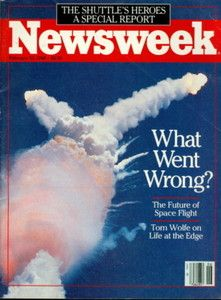
\includegraphics[width=\textwidth]{shuttle.jpg}
\end{column}
\end{columns}
\end{frame}

\begin{frame}{The evidence engineers emphasized}
Morton Thiokol engineers focused on flights with O-ring damage and worried about launching below 53$^\circ$F.
\begin{center}
\begin{tabular}{cc}
\toprule
Flight & Temperature ($^\circ$F) \\
\midrule
2 & 70 \\ 41b & 57 \\ 41c & 63 \\ 41d & 70 \\ 51c & 53 \\ 61a & 79 \\ 61c & 58 \\
\bottomrule
\end{tabular}
\end{center}
\alert{What is missing from this presentation of the data?}
\end{frame}

\begin{frame}{Selection changes the story}
Engineers considered failures, but not the successful launches.

That is \alert{selection on the dependent variable}: the failures are meaningful only when compared with the successes.

\vspace{0.5em}
Two immediate improvements:
\begin{itemize}
  \item Include all launches.
  \item Order the evidence by the explanatory variable---temperature---rather than flight number.
\end{itemize}
\end{frame}

\begin{frame}{A graph reveals the relationship}
\centering
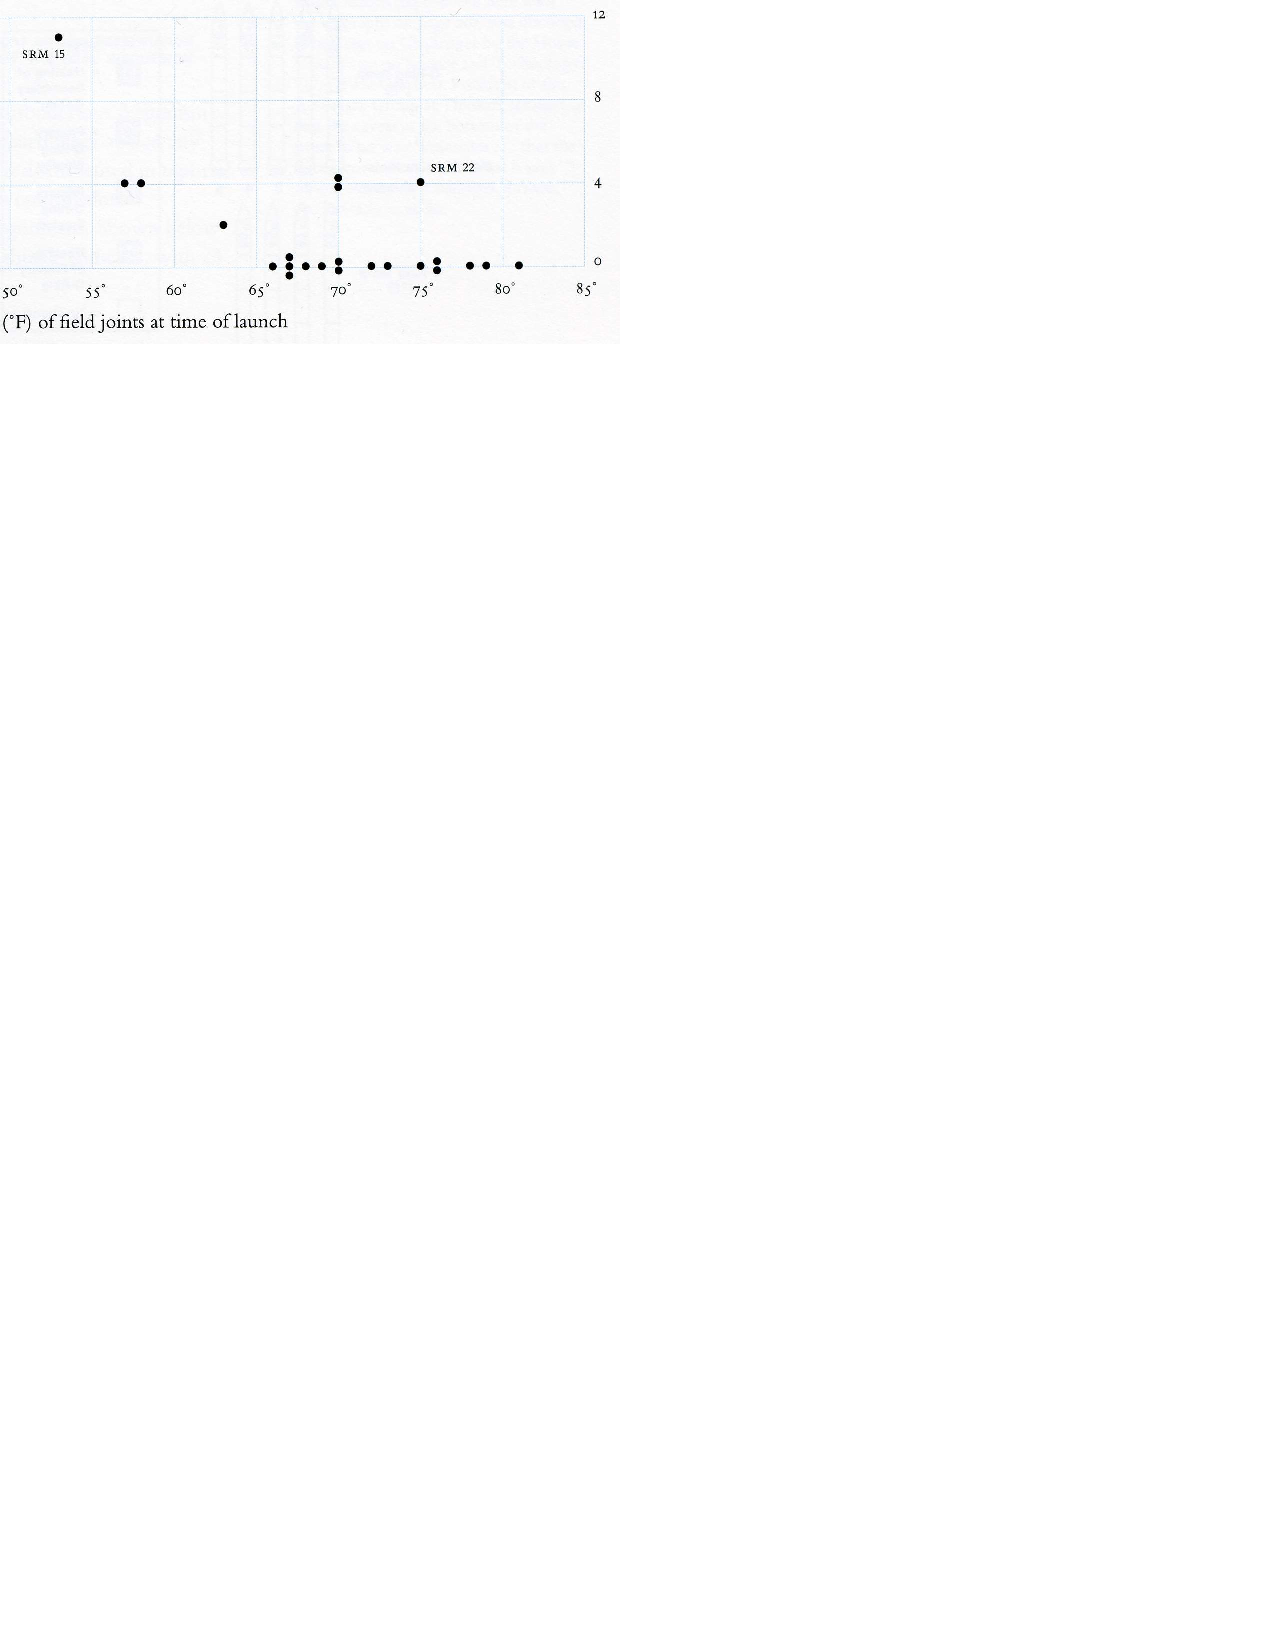
\includegraphics[width=0.82\textwidth]{tufte_challenger_1.pdf}

\small A scatterplot makes the temperature--damage relationship easier to see than a table.
\end{frame}

\begin{frame}{The launch was outside prior experience}
\centering
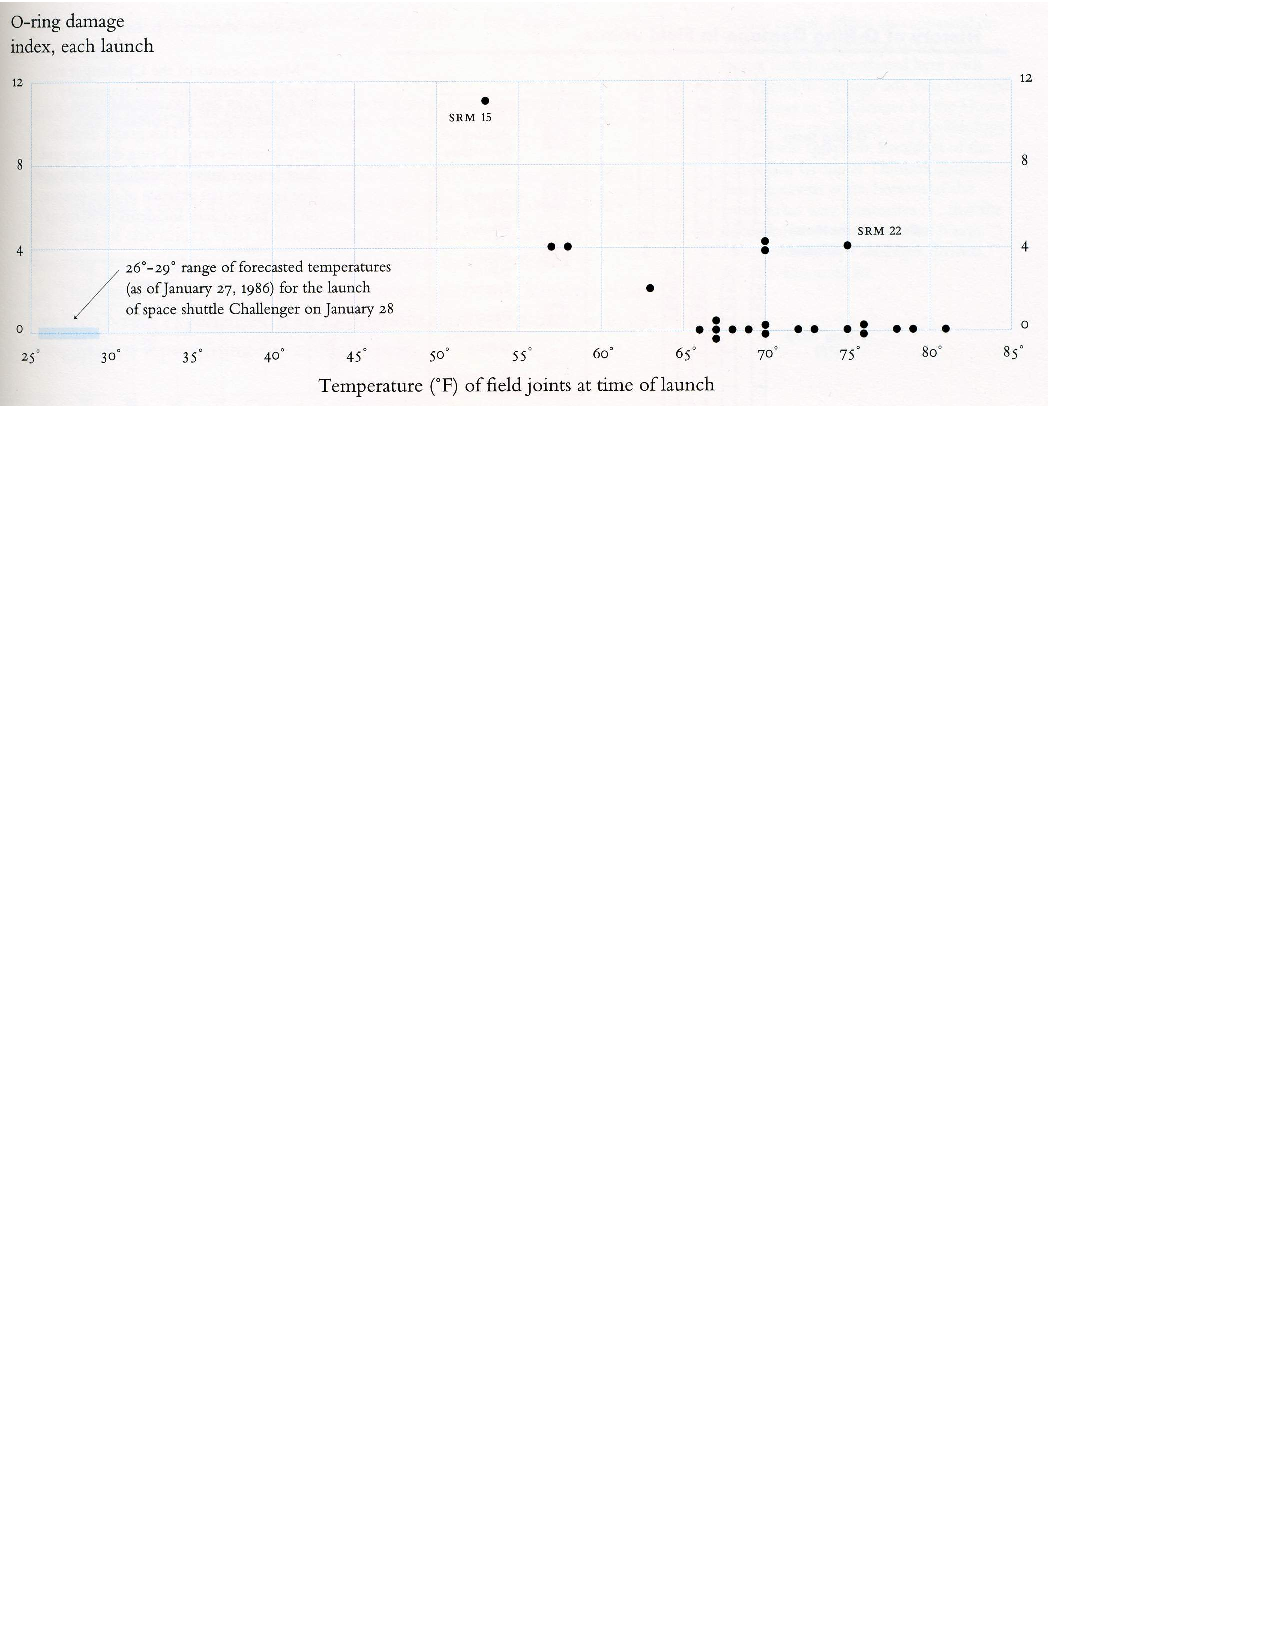
\includegraphics[width=0.82\textwidth]{tufte_challenger_2.pdf}

\small The forecast launch temperature was only 26--29$^\circ$F.
\end{frame}

\begin{frame}{From a pattern to a decision quantity}
Imagine you are making the launch recommendation. The first question is:

\begin{center}
\alert{What is the probability of O-ring damage at 29$^\circ$F?}
\end{center}

The scatterplot suggests the risk is high, but decision-makers need a more precise and communicable answer.

That requires a \textit{model}---and a clear way to present its predictions and uncertainty.
\end{frame}

\begin{frame}{Present predictions, data, and uncertainty}
\centering
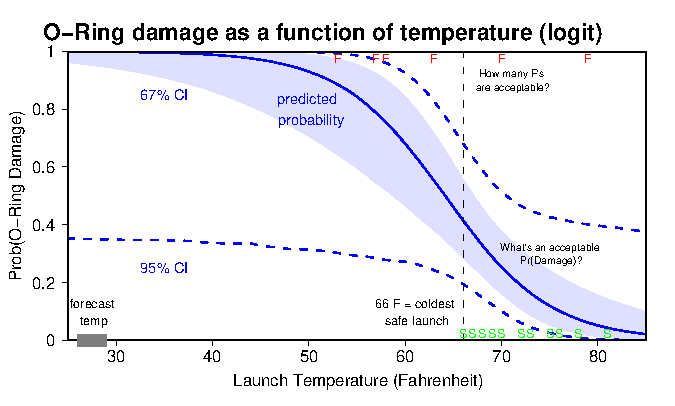
\includegraphics[width=0.68\textwidth]{chall6.pdf}

\small A useful graphic connects the observed data to model predictions and makes assumptions visible.
\end{frame}

\begin{frame}{The course in one example}
\begin{columns}
\begin{column}{0.65\textwidth}
The \textit{Challenger} case is not just about choosing a statistical method.
\begin{itemize}
  \item Ask the right question.
  \item Use all relevant data.
  \item Choose an appropriate comparison and model.
  \item Communicate the result for a consequential decision.
\end{itemize}
\end{column}
\begin{column}{0.31\textwidth}
\centering
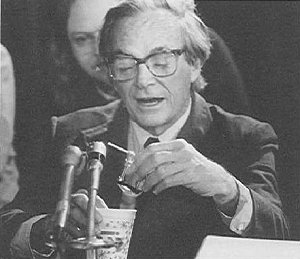
\includegraphics[width=\textwidth]{feynman.jpg}
\end{column}
\end{columns}
\end{frame}

\end{document}
